\documentclass{article}
\usepackage[utf8]{inputenc}
\usepackage{amsmath, amssymb, amsthm}
\usepackage{pgfplots}
\pgfplotsset{compat=1.18}
\usepackage{geometry}
\geometry{a4paper, margin=1in}
\usepackage{enumitem} % For custom list environments for exercises

% Custom environments for exercises
\newlist{exercises}{enumerate}{3}
\setlist[exercises]{label=\textbf{Q\arabic*.}}

\begin{document}

\title{What is 3D Calculus?}
\author{Your Academic LaTeX Expert}
\date{\today}
\maketitle

\section{Introduction to 3D Calculus}

Calculus, at its core, is the study of change. While single-variable calculus (often called 2D calculus) deals with functions of one independent variable, like $y=f(x)$, and explores concepts such as slopes of tangent lines and areas under curves, 3D calculus (also known as multivariable calculus or vector calculus) extends these ideas to functions involving multiple independent variables.

In 3D calculus, we move beyond the familiar Cartesian plane ($xy$-plane) into three-dimensional space ($xyz$-space). This allows us to model and analyze more complex real-world phenomena, such as:
\begin{itemize}
    \item The temperature distribution across a room, $T(x,y,z)$.
    \item The flow of a fluid, represented by a vector field.
    \item The gravitational force exerted by a planet, which varies with position.
    \item The volume of complex solids or the surface area of curved objects.
\end{itemize}
Essentially, 3D calculus provides the mathematical tools to understand and quantify change in a multi-dimensional world.

\section{Core Concepts of 3D Calculus}

\subsection{Functions of Multiple Variables}
Instead of $y=f(x)$, we now consider functions like $z=f(x,y)$ or $w=f(x,y,z)$.
\begin{itemize}
    \item $z=f(x,y)$: A function that takes two inputs ($x$ and $y$) and produces one output ($z$). The graph of such a function is typically a surface in 3D space.
    \item $w=f(x,y,z)$: A function that takes three inputs and produces one output. Its graph exists in 4D space, so we often visualize it using level surfaces, where $f(x,y,z)=c$ for some constant $c$.
\end{itemize}

\subsection{Partial Derivatives}
In single-variable calculus, the derivative $f'(x)$ tells us the rate of change of $f(x)$ with respect to $x$. For $f(x,y)$, we can ask how $f$ changes as we vary $x$ while holding $y$ constant, or vice-versa. This leads to partial derivatives:
\begin{itemize}
    \item $\frac{\partial f}{\partial x}$: The partial derivative of $f$ with respect to $x$, treating $y$ (and any other variables) as a constant.
    \item $\frac{\partial f}{\partial y}$: The partial derivative of $f$ with respect to $y$, treating $x$ (and any other variables) as a constant.
\end{itemize}
These represent the slopes of the surface in the $x$ and $y$ directions, respectively.

\subsection{Gradients}
The gradient of a scalar function $f(x,y,z)$ is a vector that points in the direction of the greatest rate of increase of $f$. It is denoted by $\nabla f$ (read "del f" or "nabla f"):
$$ \nabla f = \left\langle \frac{\partial f}{\partial x}, \frac{\partial f}{\partial y}, \frac{\partial f}{\partial z} \right\rangle $$
The magnitude of the gradient vector, $|\nabla f|$, gives the maximum rate of increase.

\subsection{Double and Triple Integrals}
Just as definite integrals in 2D calculus calculate areas, double and triple integrals extend this concept to higher dimensions:
\begin{itemize}
    \item \textbf{Double Integrals} ($\iint_R f(x,y) \,dA$): Used to calculate volumes under surfaces, areas of regions in the $xy$-plane, or quantities like mass or average value over a 2D region $R$.
    \item \textbf{Triple Integrals} ($\iiint_E f(x,y,z) \,dV$): Used to calculate volumes of 3D solids, mass, or average value over a 3D region $E$.
\end{itemize}

\subsection{Vector Fields}
A vector field assigns a vector to each point in space. For example, $\mathbf{F}(x,y,z) = \langle P(x,y,z), Q(x,y,z), R(x,y,z) \rangle$. Vector fields are used to model forces (gravitational, electromagnetic), fluid flow, and wind patterns.

\subsection{Line Integrals and Surface Integrals}
\begin{itemize}
    \item \textbf{Line Integrals} ($\int_C \mathbf{F} \cdot d\mathbf{r}$ or $\int_C f(x,y,z) \,ds$): Integrate a function or a vector field along a curve $C$ in space. Applications include calculating work done by a force along a path.
    \item \textbf{Surface Integrals} ($\iint_S \mathbf{F} \cdot d\mathbf{S}$ or $\iint_S f(x,y,z) \,dS$): Integrate a function or a vector field over a surface $S$ in space. Applications include calculating flux (rate of flow) through a surface.
\end{itemize}

\subsection{Fundamental Theorems of Vector Calculus}
These theorems relate different types of integrals and derivatives, providing powerful tools for solving problems:
\begin{itemize}
    \item \textbf{Green's Theorem}: Relates a line integral around a simple closed curve to a double integral over the plane region enclosed by the curve.
    \item \textbf{Stokes' Theorem}: Generalizes Green's Theorem to 3D, relating a line integral around a closed curve to a surface integral over any surface bounded by that curve.
    \item \textbf{Divergence Theorem (Gauss's Theorem)}: Relates a surface integral over a closed surface to a triple integral over the solid region enclosed by the surface.
\end{itemize}

\section{Worked Example: Analyzing a Paraboloid}

Let's consider the function $f(x,y) = x^2 + y^2$. This function describes a paraboloid, a 3D surface resembling a bowl.

\subsection{Visualizing the Surface}
The graph of $z = x^2 + y^2$ is shown below. Notice how the value of $z$ increases as $x$ or $y$ move away from the origin.

\begin{figure}[htbp]htbp]
    \centering
    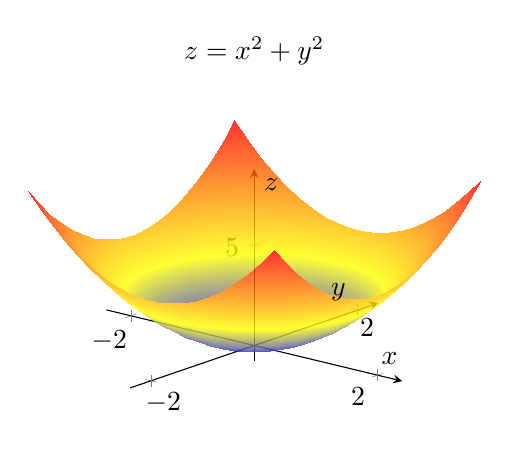
\begin{tikzpicture}
        \begin{axis}[
            title={$z = x^2 + y^2$},
            xlabel={$x$},
            ylabel={$y$},
            zlabel={$z$},
            axis lines=middle,
            enlargelimits=true,
            width=0.7\textwidth,
            height=6cm,
            view={40}{30} % Adjust view angle for better perspective
        ]
            \addplot3[
                surf,
                domain=-2:2,
                y domain=-2:2,
                samples=20, % Number of samples for smoother surface
                shader=interp, % Smooth color interpolation
                opacity=0.8,
                z buffer=sort % Correct rendering for overlapping surfaces
            ] {x^2 + y^2};
        \end{axis}
    \end{tikzpicture}
    \caption{Graph of the paraboloid $z = x^2 + y^2$.}
\end{figure}

\subsection{Partial Derivatives}
Let's find the partial derivatives of $f(x,y) = x^2 + y^2$:
\begin{itemize}
    \item To find $\frac{\partial f}{\partial x}$, we treat $y$ as a constant:
    $$ \frac{\partial f}{\partial x} = \frac{\partial}{\partial x}(x^2 + y^2) = 2x + 0 = 2x $$
    This tells us that if we move in the positive $x$-direction (holding $y$ constant), the slope of the surface is $2x$.
    \item To find $\frac{\partial f}{\partial y}$, we treat $x$ as a constant:
    $$ \frac{\partial f}{\partial y} = \frac{\partial}{\partial y}(x^2 + y^2) = 0 + 2y = 2y $$
    Similarly, moving in the positive $y$-direction (holding $x$ constant), the slope is $2y$.
\end{itemize}

\subsection{Gradient}
The gradient of $f(x,y) = x^2 + y^2$ is:
$$ \nabla f = \left\langle \frac{\partial f}{\partial x}, \frac{\partial f}{\partial y} \right\rangle = \langle 2x, 2y \rangle $$
At a point like $(1,1)$, the gradient is $\nabla f(1,1) = \langle 2(1), 2(1) \rangle = \langle 2, 2 \rangle$. This vector points in the direction of the steepest ascent on the paraboloid at $(1,1)$.

\subsection{Double Integral (Volume)}
Let's set up a double integral to find the volume under the surface $z = x^2 + y^2$ over the rectangular region $R = [0,1] \times [0,1]$ (i.e., $0 \le x \le 1$ and $0 \le y \le 1$).
The volume $V$ is given by:
$$ V = \iint_R (x^2 + y^2) \,dA = \int_0^1 \int_0^1 (x^2 + y^2) \,dx \,dy $$
First, integrate with respect to $x$:
$$ \int_0^1 (x^2 + y^2) \,dx = \left[ \frac{x^3}{3} + xy^2 \right]_0^1 = \left( \frac{1^3}{3} + (1)y^2 \right) - \left( \frac{0^3}{3} + (0)y^2 \right) = \frac{1}{3} + y^2 $$
Now, integrate the result with respect to $y$:
$$ V = \int_0^1 \left( \frac{1}{3} + y^2 \right) \,dy = \left[ \frac{1}{3}y + \frac{y^3}{3} \right]_0^1 = \left( \frac{1}{3}(1) + \frac{1^3}{3} \right) - \left( \frac{1}{3}(0) + \frac{0^3}{3} \right) = \frac{1}{3} + \frac{1}{3} = \frac{2}{3} $$
So, the volume under the paraboloid $z=x^2+y^2$ over the unit square is $\frac{2}{3}$ cubic units.

\section{Exercises}

\begin{exercises}
    \item \textbf{Level 1: Basic Understanding}
    Given the function $f(x,y) = 3x^2y - 5xy^3 + 7$, find the partial derivatives $\frac{\partial f}{\partial x}$ and $\frac{\partial f}{\partial y}$.
    \begin{proof}
        To find $\frac{\partial f}{\partial x}$, treat $y$ as a constant:
        $$ \frac{\partial f}{\partial x} = \frac{\partial}{\partial x}(3x^2y) - \frac{\partial}{\partial x}(5xy^3) + \frac{\partial}{\partial x}(7) = 3y \cdot (2x) - 5y^3 \cdot (1) + 0 = 6xy - 5y^3 $$
        To find $\frac{\partial f}{\partial y}$, treat $x$ as a constant:
        $$ \frac{\partial f}{\partial y} = \frac{\partial}{\partial y}(3x^2y) - \frac{\partial}{\partial y}(5xy^3) + \frac{\partial}{\partial y}(7) = 3x^2 \cdot (1) - 5x \cdot (3y^2) + 0 = 3x^2 - 15xy^2 $$
    \end{proof}

    \item \textbf{Level 2: Application/Conceptual}
    Calculate the gradient of the function $g(x,y,z) = x \sin(yz)$ at the point $(1, \pi/2, 1)$.
    \begin{proof}[Hint]
        Recall that the gradient of a scalar function $g(x,y,z)$ is given by the vector $\nabla g = \left\langle \frac{\partial g}{\partial x}, \frac{\partial g}{\partial y}, \frac{\partial g}{\partial z} \right\rangle$. Calculate each partial derivative, then substitute the given point $(1, \pi/2, 1)$ into the resulting expressions. Remember the chain rule for derivatives involving $yz$.
    \end{proof}

    \item \textbf{Level 3: Advanced/Problem Solving}
    A thin plate occupies the region $D$ in the $xy$-plane bounded by the curves $y=x^2$ and $y=x+2$. If the density of the plate at any point $(x,y)$ is given by $\rho(x,y) = x^2y$, set up (but do not evaluate) the double integral for the total mass of the plate.
\end{exercises}

\end{document}